\documentclass[12pt, a4paper]{article}

\usepackage[ngerman]{babel} 
\usepackage[T1]{fontenc}
\usepackage{amsfonts} 
\usepackage{setspace}
\usepackage{amsmath}
\usepackage{amssymb}
\usepackage{tikz}
\usepackage{titling}

\graphicspath{./}

\newcommand*{\qed}{\null\nobreak\hfill\ensuremath{\square}}
\newcommand*{\puffer}{\text{ }\text{ }\text{ }\text{ }}
\newcommand*{\lhop}{\mathrel{\overset{\makebox[0pt]{\mbox{\normalfont\tiny\sffamily l'hop.}}}{=}}}

\pagestyle{plain}
\allowdisplaybreaks

\setlength{\droptitle}{-10em}

\title{Einführung in die Algorithmik - Hausaufgabenserie 7}
\author{Nike Pulow, Henri Heyden\\ \small stu239549, stu240825}
\date{}


\begin{document}
\maketitle
\section*{Aufgabe 2}
\subsection*{c)}
Zu betrachten ist der source-code für diese Teilaufgabe. \\
Die Ausgabe des Programms haben wir in einer Grafik dargestellt:\\
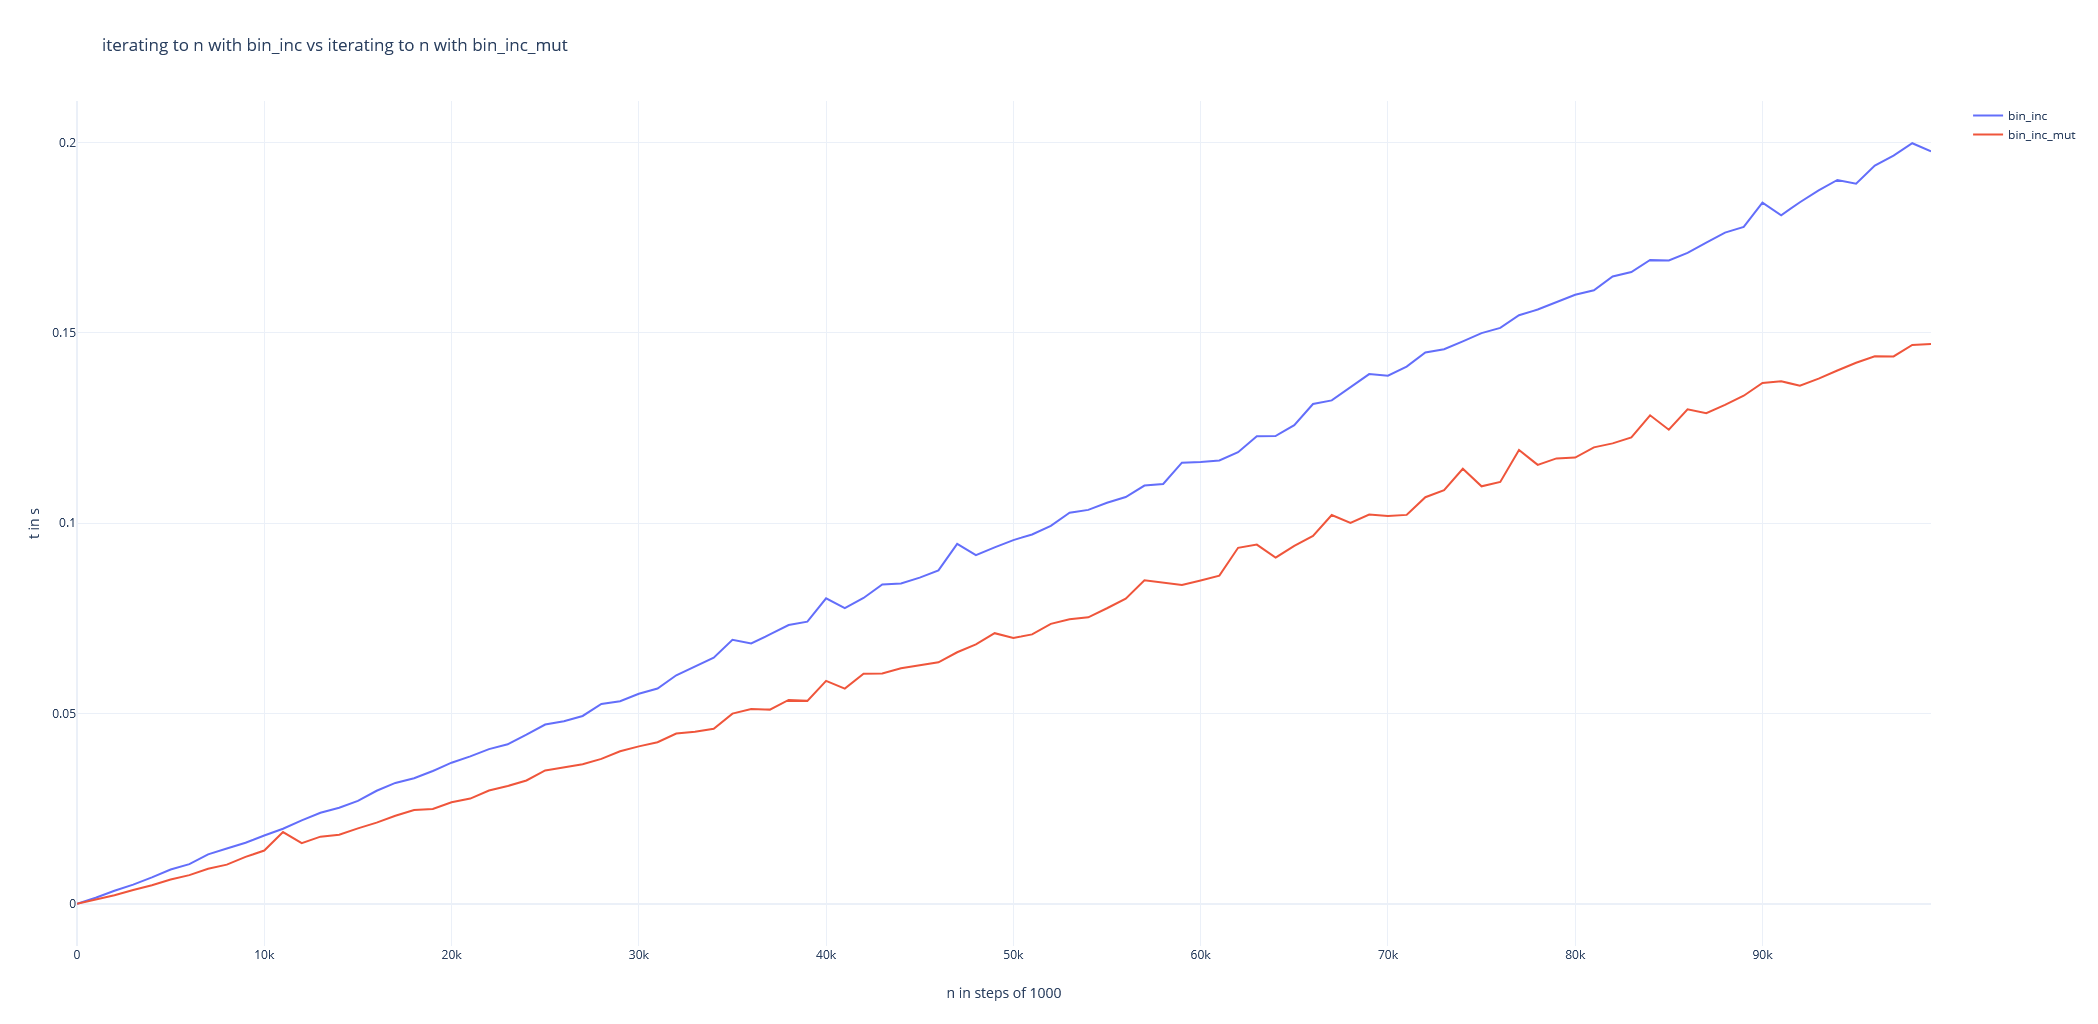
\includegraphics[width=\textwidth]{DiagramFor7.2.png}
Hier haben wir die Zeiten, die das Programm für mehrere \(n \in [0, 100000]\) dargestellt mit einer Genauigkeit von 100 Eingaben pro Methode mit 1000 großen Stufen zwischen den Schritten. \\
Die Resultate aus den vorherigen Aufgaben scheinen sich auch in dieser empirischen Messung widerzuspiegeln, denn die Graphen sehen sehr linear aus. \\
Sie haben dabei ungefähr Steigungen von \( 1.996496909 \cdot 10^{-6} s\setminus n\) und \( 1.485328283 \cdot 10^{-6} s\setminus n\) \\
Wenn man die Steigungen durch einander teilt, ergibt sich, dass bin\_inc\_mut um einen Faktor \( 1.490549815 \) schneller ist als bin\_inc. \\
Wie schon erwähnt halt bin\_inc\_mut den Vorteil, dass es abbrechen kann, wenn es realisiert, dass keine Additionen mehr ausgeführt werden müssen, währenddessen bin\_inc alle restlichen Elemente noch kopieren muss. Dieser bessere average case taucht immer genau nach einem worst case auf, denn nachdem eine Zahl, die eine sehr lange kette an Einsen am Anfang hat inkrementiert wurde, verwandeln sich diese vielen Einsen in Nullen und wir haben konstante Laufzeit und dannach langsam mehr Laufzeit bis zum Maximum n. \\
Es gibt mehr best case Szenarien bei bin\_inc\_mut als bei bin\_inc, und der average case von bin\_inc ist ähnlich zu dem worst case von bin\_inc\_mut. Ungefähr gibt es 50 Prozent der Fälle einen solchen besseren Fall bei bin\_inc\_mut, weswegen auch bin\_inc\_mut nach Messung fast um 150 Prozent schneller ist.
Insgesamt werden also ein Faktor von n weniger Operationen ausgeführt.
\subsection*{d)}
Zu betrachten ist wieder der source-code für diese Teilaufgabe. \\
Wir haben uns eine Helfermethode geschrieben, um für die Zahlen 0 bis 1000 herauszufinden, wie viele Operationen verwendet werden müssen. \\
Die Ausgabe des Programms haben wir in einer Grafik dargestellt:\\
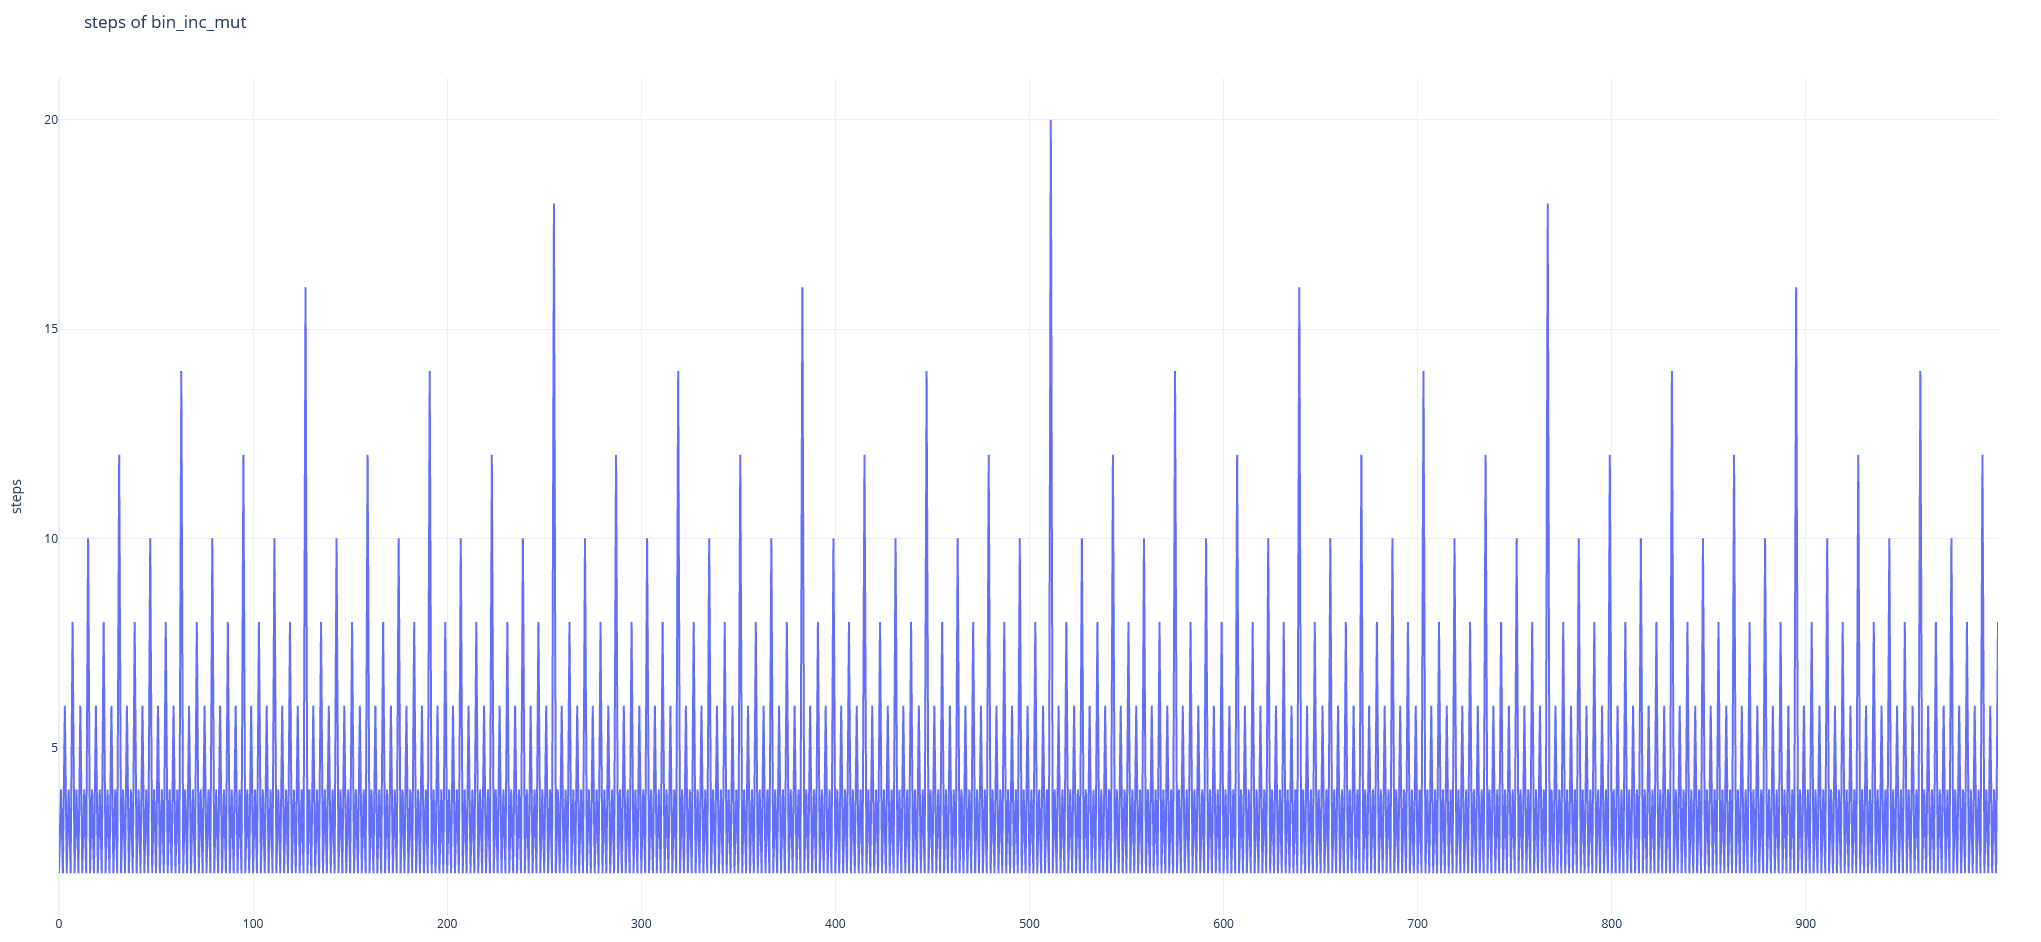
\includegraphics[width=\textwidth]{DiagramFor7.2.4.png}
Ich finde, der Graph sieht ein bisschen aus, wie ein Binärbaum... \\
Wenn man ein bisschen mehr hineinzoomt (die Daten für den Plot sind auch im sourcecode) sieht man, dass das Minimum 2 Operationen ist, welches genau jedes zweite Mal auftritt. Dies ergibt Sinn, da natürlich im Binärsystem das LSB bei Iteration immer zwischen 0 und 1 wechselt. \\
Die höhere Stufe ist 4 Operationen, welche jedes vierte Mal auftreten, dies ist der Fall, dass die letzten (in unseren Listen die ersten) zwei Bits 1 sind (und dannach dann eine 0 folgt), da dann sich das Carry Bit zur dritten Stelle überträgt. \\
Die worst cases oder auch bad average cases enstehen immer, wenn das Carry Bit auf Folgen von Einsen anfangend beim LSB trifft. Hier ist die Anzahl an extra Schritten proportional zu der Anzahl an Einsen, die direkt auf das LSB folgen. \pagebreak \\
Aus diesen Beobachtungen ergibt sich folgender Schluss: Die Anzahl der Schritte des Inkrementierens ist amortisiert höchstens \(2 \cdot \log_2 (n + 1) + 2\), da das Programm mindestens 2 Schritte machen muss, und pro Wiederholung genau 2 Schritte hinzukommen. \\
Wir kommen auf \(n + 1\) in dem Term, da der worst case immer auftritt, wenn wir genau eine Zahl vor einer Zweierpotenz sind. \\
Wir können also sagen, dass im worst case bin\_inc\_mut amortisiert die Landauklasse \(\mathcal O(2\cdot log_n(n+1) + 2) = O(2\cdot log_n(n+1)) = O(log_n(n+1)) = O(log_n(n))\) besitzt.
\end{document}